\subsubsection{Умножитель напряжения}

Схема, позволяющая получить из переменного тока постоянный, напряжение которого в несколько раз больше чем у исходного переменного.

\begin{center}
	\begin{figure}[H]
		\center{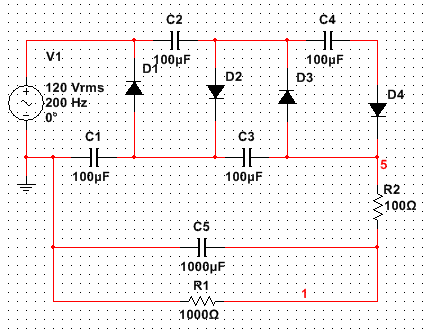
\includegraphics[scale=0.9]{V_mult.png}}
		\caption{Схема умножителя напряжения}
	\end{figure}
\end{center} 


\begin{center}
	\begin{figure}[H]
		\center{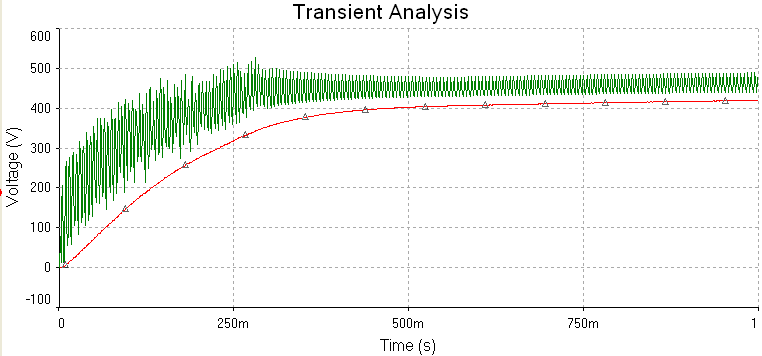
\includegraphics[scale=0.9]{mult_trans.png}}
		\caption{Временная характеристика забыты схемы}
	\end{figure}
\end{center} 

Суть работы такова:
\begin{itemize}
\item Через диод D1 конденсатор C1 заряжается максимально до E
\item При обратной полуволне через диод D2 заряжается конденсатор C2, при этом контур зарядки содержит предварительно заряженный конденсатор C1, следовательно, максимальное напряжение до которого о может зарядиться = 2E, без учета падения напряжения на диодах.
\item etc.
\item PROFIT!
\end{itemize}

